\section{Transformation framework}

\begin{frame}{How to transform this type model...}
    \centering
    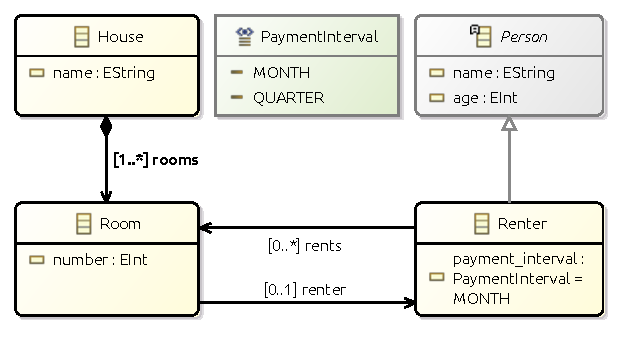
\includegraphics[trim={0 0.45cm 0 0.25cm},clip]{images/02_modelling_languages/type_model_example.pdf}
\end{frame}

\begin{frame}{...into this type graph}
    \centering
    % To use this figure in your LaTeX document
% import the package groove/resources/groove2tikz.sty
%
\begin{tikzpicture}[scale=\tikzscale,name prefix=type-]
\node[type_node] (n0) at (0.560, -0.290) {\ml{\textbf{House}\\name: \textbf{string}}};
\node[type_node] (n1) at (0.600, -1.430) {\ml{\textbf{Room}\\number: \textbf{int}}};
\node[type_node] (n2) at (2.470, -1.435) {\ml{\textbf{Renter}}};
\node[type_node] (n3) at (2.470, -2.175) {\ml{\textit{\textbf{PaymentInterval}}}};
\node[type_node] (n4) at (1.170, -2.785) {\ml{\textbf{PaymentInterval\$MONTH}}};
\node[type_node] (n5) at (3.830, -2.785) {\ml{\textbf{PaymentInterval\$QUARTER}}};
\node[type_node] (n6) at (2.470, -0.375) {\ml{\textit{\textbf{Person}}\\age: \textbf{int}\\name: \textbf{string}}};

\path[subtype_edge](n2.north -| 2.470, -0.375) --  (n6) ;
\path[subtype_edge] (n4)  --  (n3) ;
\path[subtype_edge] (n5)  --  (n3) ;
\path[basic_edge](n2.west |- 0.600, -1.430) -- node[lab] {\ml{rents}} (n1) ;
\path[basic_edge, composite](n0.south -| 0.600, -1.430) -- node[lab] {\ml{rooms}} (n1) ;
\path[basic_edge](n2.south -| 2.470, -2.175) -- node[lab] {\ml{payment\_interval}} (n3) ;
\path[basic_edge](n1.east |- 2.470, -1.435) -- node[lab] {\ml{renter}} (n2) ;
\end{tikzpicture}

\end{frame}

\begin{frame}{And what about transforming this instance model...}
    \centering
    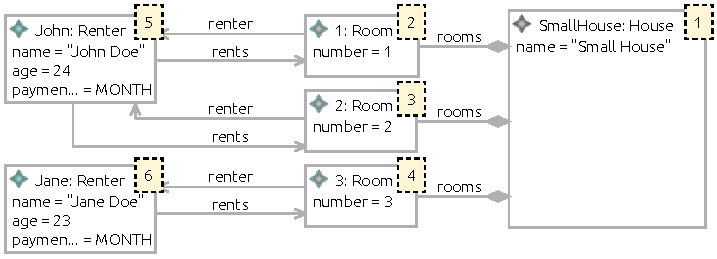
\includegraphics[]{images/02_modelling_languages/instance_model_example.pdf}
\end{frame}

\begin{frame}{...into this instance graph}
    \centering
    % To use this figure in your LaTeX document
% import the package groove/resources/groove2tikz.sty
%
\begin{tikzpicture}[scale=\tikzscale,name prefix=start-]
\node[basic_node] (n0) at (2.235, -0.335) {\ml{\uline{\textit{Renter1}} : \textbf{Renter}\\age = 24\\name = "J.A."}};
\node[basic_node] (n1) at (2.225, -2.305) {\ml{\uline{\textit{Renter2}} : \textbf{Renter}\\age = 23\\name = "M.S."}};
\node[basic_node] (n2) at (1.005, -1.345) {\ml{\textbf{PaymentInterval\$MONTH}}};
\node[basic_node] (n3) at (4.605, -0.330) {\ml{\uline{\textit{Longhorn}} : \textbf{Room}\\number = 1}};
\node[basic_node] (n4) at (4.585, -1.370) {\ml{\uline{\textit{Shorthorn}} : \textbf{Room}\\number = 2}};
\node[basic_node] (n5) at (4.595, -2.330) {\ml{\uline{\textit{onghornLay}} : \textbf{Room}\\number = 3}};
\node[basic_node] (n6) at (6.975, -1.380) {\ml{\uline{\textit{TwoRem}} : \textbf{House}\\name = "Small House"}};

\path[basic_edge] (n6)  -- node[lab] {\ml{rooms}} (n5) ;
\path[basic_edge](n6.west |- 4.585, -1.370) -- node[lab] {\ml{rooms}} (n4) ;
\path[basic_edge](n3.west |- 2.235, -0.235) -- node[lab] {\ml{renter}} (n0) ;
\path[basic_edge] (n4.west)  -- node[lab] {\ml{renter}} (n0) ;
\path[basic_edge](n5.west |- 2.225, -2.205) -- node[lab] {\ml{renter}} (n1) ;
\path[basic_edge] (n0)  -- node[lab] {\ml{payment\_interval}} (n2) ;
\path[basic_edge] (n6)  -- node[lab] {\ml{rooms}} (n3) ;
\path[basic_edge] (n0) -- node[lab] {\ml{rents}} (n3.west |- 4.605, -0.430) ;
\path[basic_edge] (n1)  -- node[lab] {\ml{payment\_interval}} (n2) ;
\path[basic_edge](n1) -- node[lab] {\ml{rents}} (n5.west |- 4.595, -2.430) ;
\path[basic_edge] (n0)  -- node[lab] {\ml{rents}} (n4.north) ;
\end{tikzpicture}

\end{frame}

\begin{frame}{Transformation framework}
    \begin{itemize}
        \item There exist infinitely many possible models and graphs.
        \item As a consequence, there are infinitely many possible model transformations.\pause
        \item Conclusion: It is not possible to separately proof all of them.
    \end{itemize}
    \vspace{1cm}
    How to solve this issue?
\end{frame}

\note{
	\begin{itemize}
	    \item Explain that the problem is not trivial, especially since correctness needs to be proven.
	    \item Explain that the approach is key, as it is impossible to have a proof for all possible model transformations.
	    \item Cliffhanger: How to solve the issue of infinitely many model transformations.
	\end{itemize}
}

\begin{frame}<1-2>[label=framework]{Transformation framework}
    What if transformations and their proofs can be composed? \pause
    \begin{itemize}
        \item The well-known concept of divide and conquer
        \item Use small additions to a model to create a larger model. \pause
        \item Give the 'small additions' a corresponding transformation.
        \item Apply small additions in both languages at the same time, create a larger model transformation with each step.
    \end{itemize}
\end{frame}

\begin{frame}{Combining models}
    The concept of building models out of small parts... \pause
    We have seen that before!
    \begin{columns}[c]
        \begin{column}{0.05\textwidth}
        \end{column}\begin{column}{0.35\textwidth}
            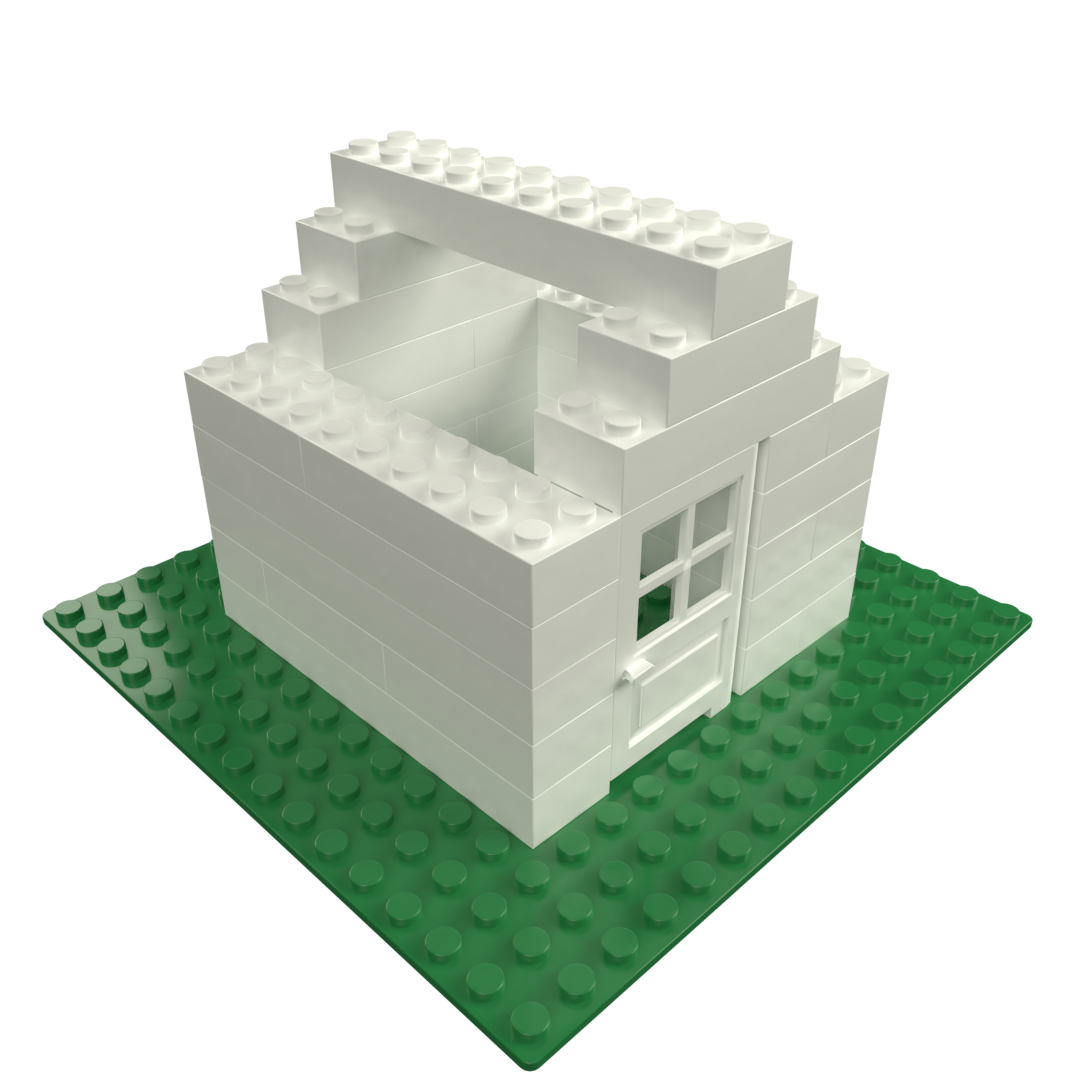
\includegraphics[width=\textwidth]{images/03_transformation_framework/lego_house_roofless.png}
        \end{column}\begin{column}{0.2\textwidth}
            
\includegraphics[width=\textwidth]{images/03_transformation_framework/lego_roof_pieces.png}
        \end{column}\begin{column}{0.35\textwidth}
            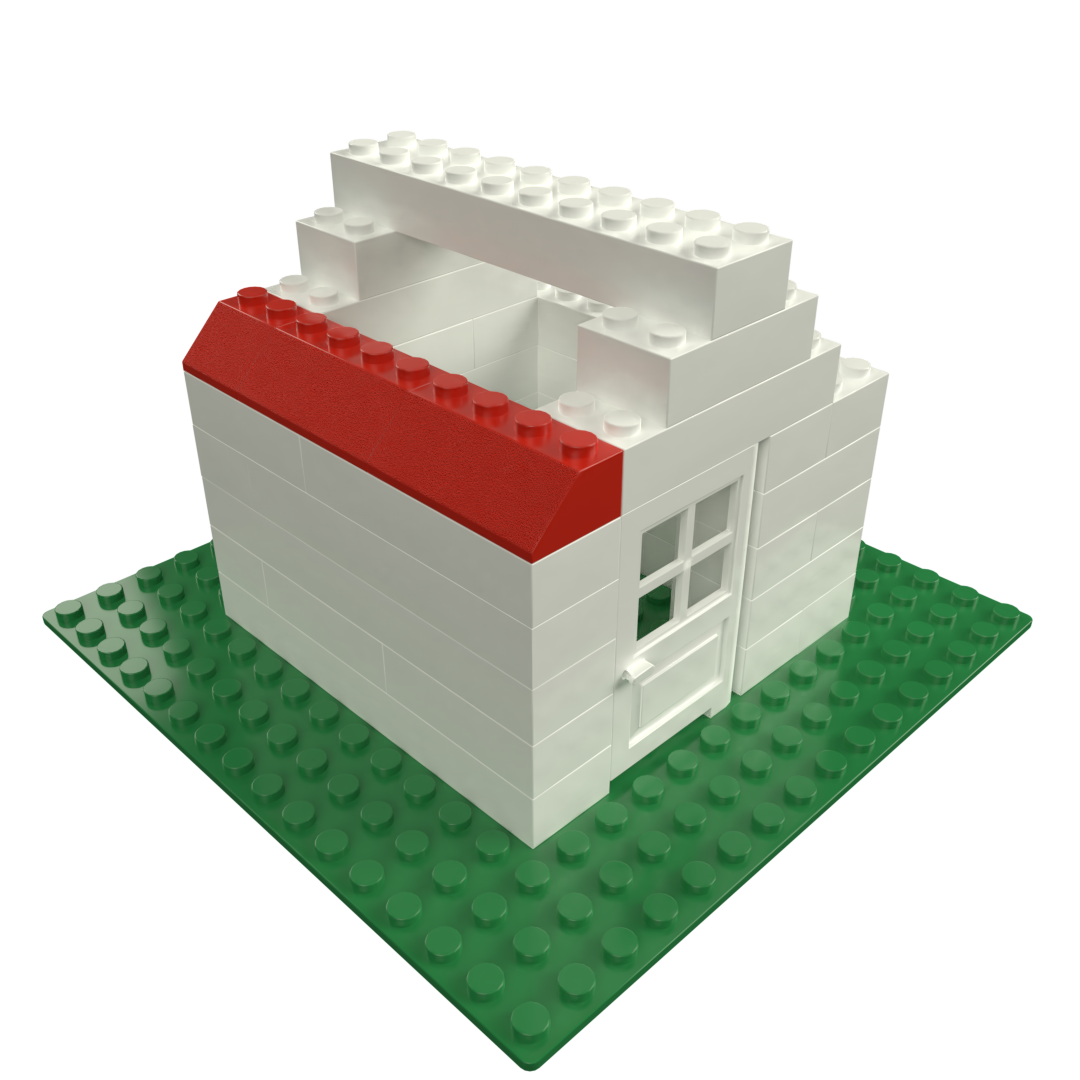
\includegraphics[width=\textwidth]{images/03_transformation_framework/lego_house_roof_step.png}
        \end{column}
    \end{columns} 
\end{frame}

\againframe<3>{framework}

\note{
	\begin{itemize}
	    \item Roughly explain that building the models iteratively is key.
	    \item This concept is also known from Lego!
	    \item These small steps are easier to create correctness proofs for.
	    \item Small steps can be combined over and over, as a way to create correct model transformations.
	\end{itemize}
}

\begin{frame}{Structure}
    \centering
    \begin{tikzpicture} 
    \path
    (-3,4) node[circle,draw,minimum size=10mm,inner sep=0pt](ME) {$E$}
    (-4.5,2) node[circle,draw,minimum size=10mm,inner sep=0pt](MA) {$M_A$}
    (-1.5,2) node[circle,draw,minimum size=10mm,inner sep=0pt](MB) {$M_B$}
    (-3,0) node[circle,draw,minimum size=10mm,inner sep=0pt](MAB) {$M_{AB}$}
    
    (3,4) node[circle,draw,minimum size=10mm,inner sep=0pt](GN) {$N$}
    (1.5,2) node[circle,draw,minimum size=10mm,inner sep=0pt](GA) {$G_A$}
    (4.5,2) node[circle,draw,minimum size=10mm,inner sep=0pt](GB) {$G_B$}
    (3,0) node[circle,draw,minimum size=10mm,inner sep=0pt](GAB) {$G_{AB}$};
    
    \path[]		
    (ME) [-, black, out=240, in=90] edge node[above] {} (MA)
    (ME) [-, black, out=300, in=90] edge node[above] {} (MB)
    
    (MA) [-{Latex[width=5]}, black, out=270, in=90] edge node[above] {} (MAB)
    (MB) [-{Latex[width=5]}, black, out=270, in=90] edge node[above] {} (MAB)
    
    (GN) [-, black, out=240, in=90] edge node[above] {} (GA)
    (GN) [-, black, out=300, in=90] edge node[above] {} (GB)
    
    (GA) [-{Latex[width=5]}, black, out=270, in=90] edge node[above] {} (GAB)
    (GB) [-{Latex[width=5]}, black, out=270, in=90] edge node[above] {} (GAB)
    
    (ME) [-{Latex[width=5]}, black, out=25, in=155] edge node[above] {$f$} (GN)
    (GN) [-{Latex[width=5]}, black, out=165, in=15] edge node[above] {} (ME)
    
    (MA) [-{Latex[width=5]}, black, out=35, in=145] edge node[above] {$f_A$} (GA)
    (GA) [-{Latex[width=5]}, black, out=155, in=25] edge node[above] {} (MA)
    
    (MB) [-{Latex[width=5]}, black, out=35, in=145] edge node[above] {$f_B$} (GB)
    (GB) [-{Latex[width=5]}, black, out=155, in=25] edge node[above] {} (MB)
    
    (MAB) [-{Latex[width=5]}, black, out=25, in=155] edge node[above] {$f_{A} \sqcup f_{B}$} (GAB)
    (GAB) [-{Latex[width=5]}, black, out=165, in=15] edge node[above] {} (MAB)
    ;
    \end{tikzpicture}
\end{frame}

\note{
	\begin{itemize}
	    \item Explain on an abstract level what the transformation framework is.
	    \item Make clear that when applying steps to the model side, a similar step is applied to the graph side.
	    \item Similar means, there is a correct transformation between the added steps.
	\end{itemize}
}

\begin{frame}{Combining transformations}
\begin{columns}[c]
    \begin{column}{0.05\textwidth}
    \end{column}\begin{column}{0.3\textwidth}
        
\includegraphics[width=\textwidth]{images/02_modelling_languages/lego_house.png}
    \end{column}\begin{column}{0.45\textwidth}
        \centering
        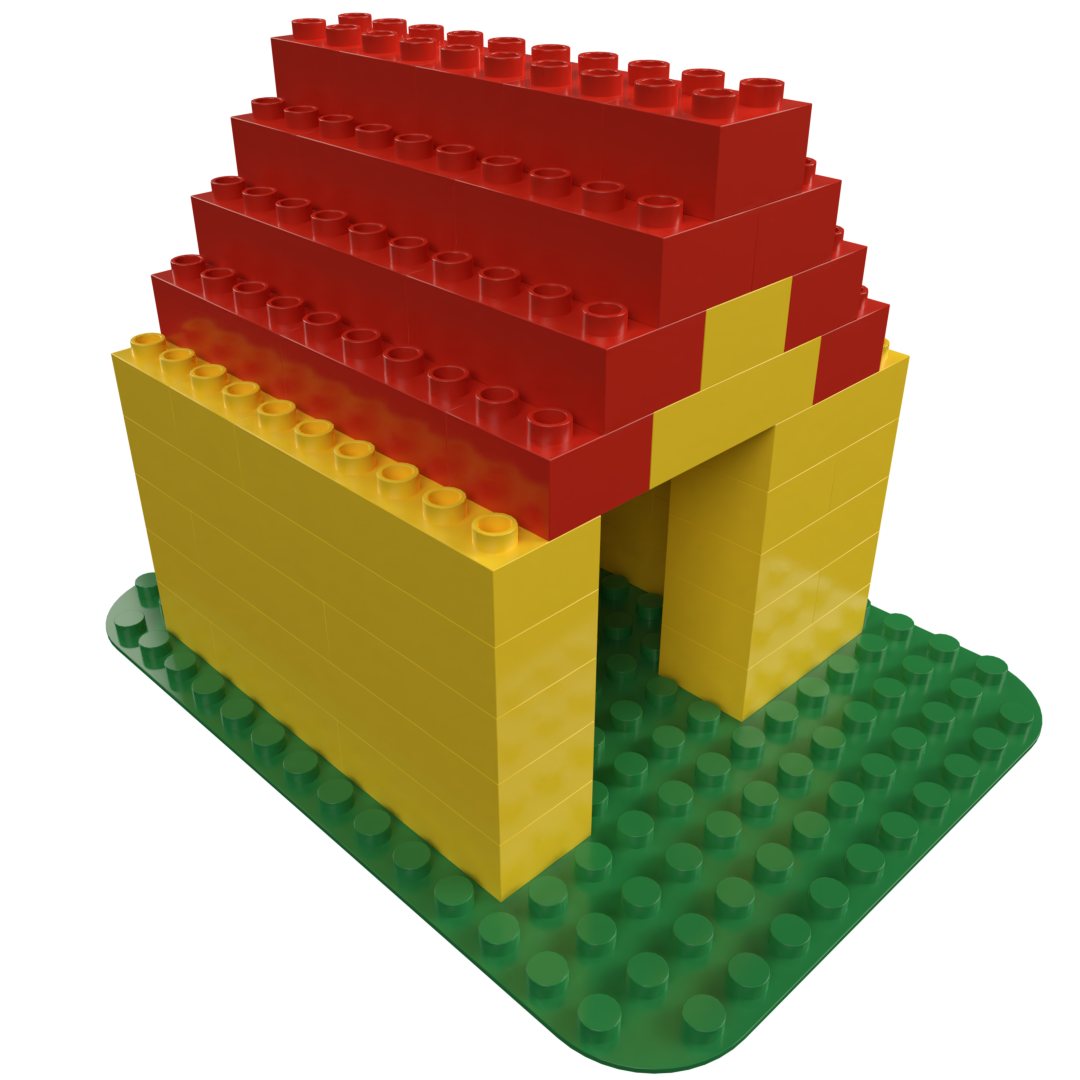
\includegraphics[width=\textwidth]{images/03_transformation_framework/duplo_house.png}
    \end{column}
\end{columns}
\end{frame}

\begin{frame}{Combining transformations}
    \begin{columns}[c]
        \begin{column}{0.05\textwidth}
        \end{column}\begin{column}{0.3\textwidth}
            \centering
            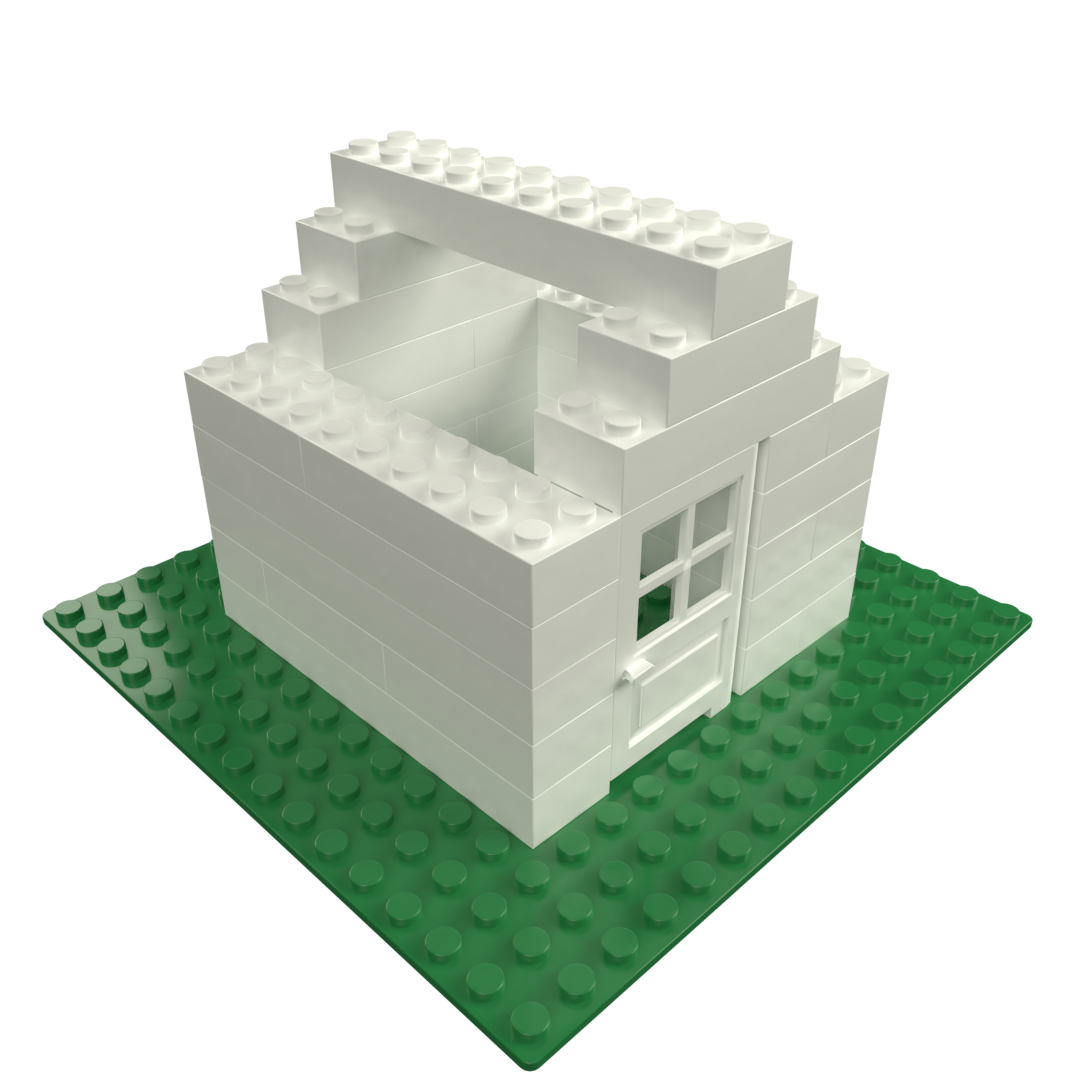
\includegraphics[width=0.7\textwidth]{images/03_transformation_framework/lego_house_roofless.png}
        \end{column}\begin{column}{0.05\textwidth}
            \centering
            +
        \end{column}\begin{column}{0.2\textwidth}
            \centering
            
\includegraphics[width=0.7\textwidth]{images/03_transformation_framework/lego_roof_pieces.png}
        \end{column}\begin{column}{0.05\textwidth}
            \centering
            =
        \end{column}\begin{column}{0.3\textwidth}
            \centering
            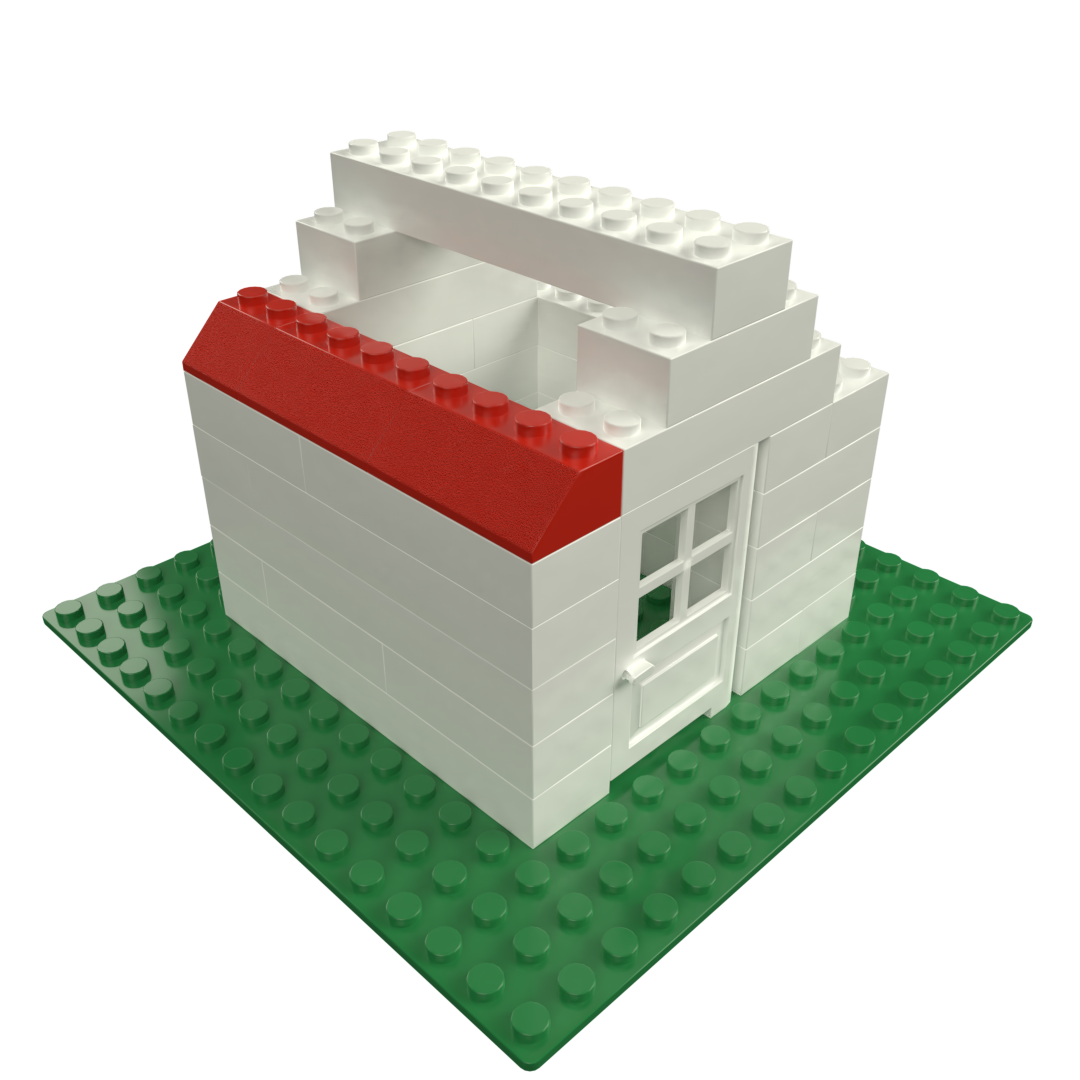
\includegraphics[width=0.7\textwidth]{images/03_transformation_framework/lego_house_roof_step.png}
        \end{column}
    \end{columns}
    \begin{columns}[c]
        \begin{column}{0.05\textwidth}
        \end{column}\begin{column}{0.3\textwidth}
            \centering
            \rotatebox{90}{$\leftrightarrow$}
        \end{column}\begin{column}{0.05\textwidth}
            \centering
            $\sqcup$
        \end{column}\begin{column}{0.2\textwidth}
            \centering
            \rotatebox{90}{$\leftrightarrow$}
        \end{column}\begin{column}{0.05\textwidth}
            \centering
            =
        \end{column}\begin{column}{0.3\textwidth}
            \centering
            \rotatebox{90}{$\leftrightarrow$}
        \end{column}
    \end{columns} 
    \begin{columns}[c]
        \begin{column}{0.05\textwidth}
        \end{column}\begin{column}{0.3\textwidth}
            \centering
            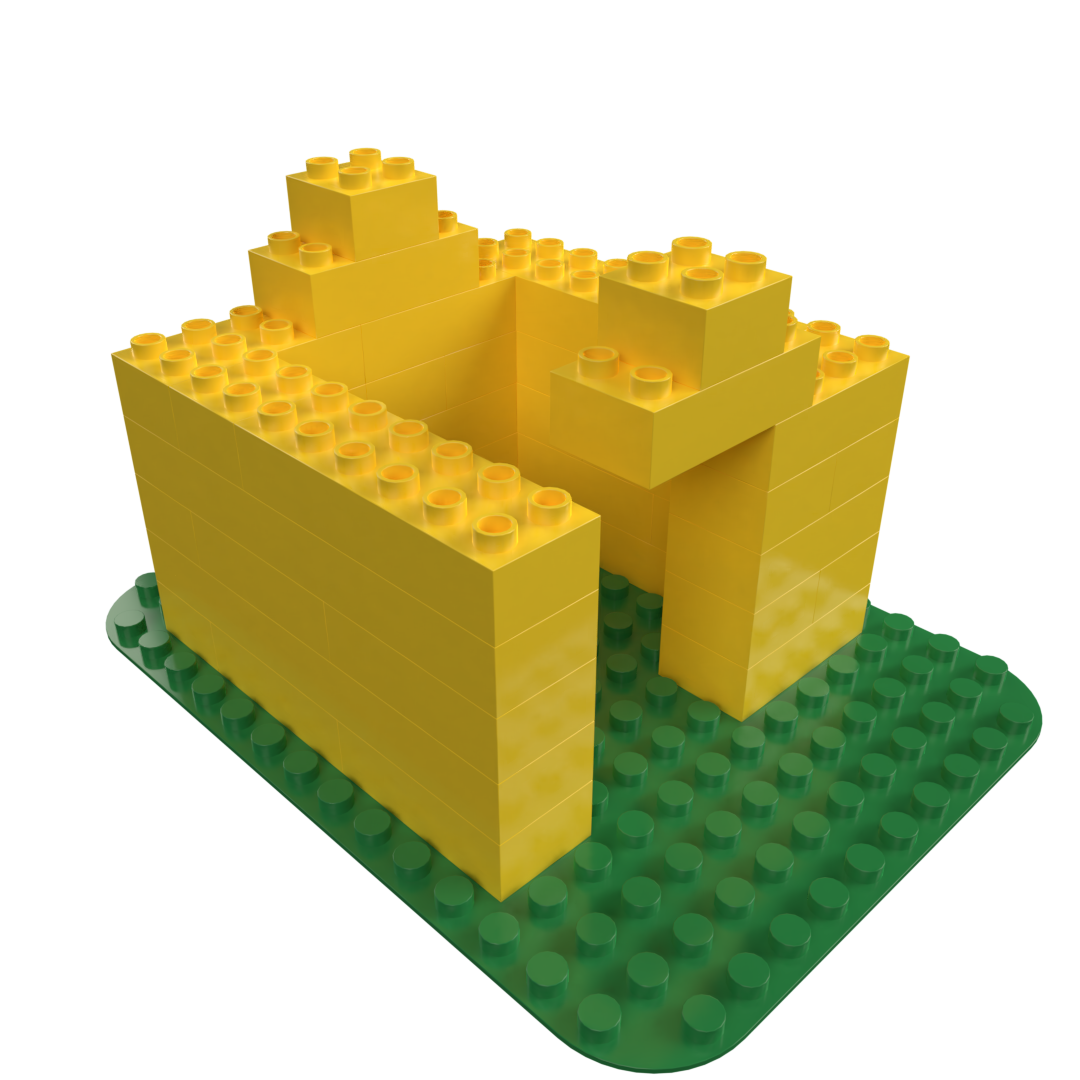
\includegraphics[width=0.7\textwidth]{images/03_transformation_framework/duplo_house_roofless.png}
        \end{column}\begin{column}{0.05\textwidth}
            \centering
            +
        \end{column}\begin{column}{0.2\textwidth}
            \centering
            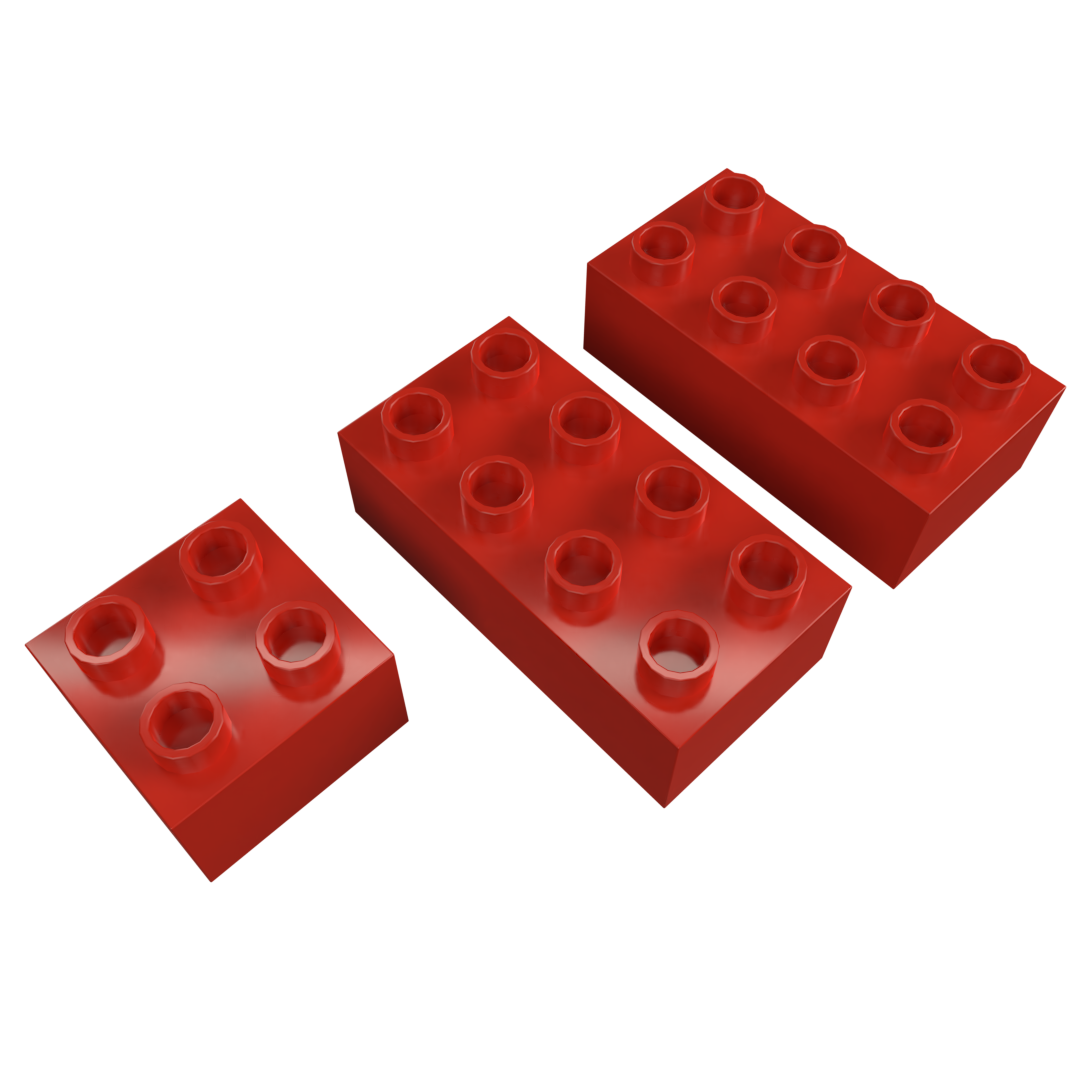
\includegraphics[width=0.7\textwidth]{images/03_transformation_framework/duplo_roof_pieces.png}
        \end{column}\begin{column}{0.05\textwidth}
            \centering
            =
        \end{column}\begin{column}{0.3\textwidth}
            \centering
            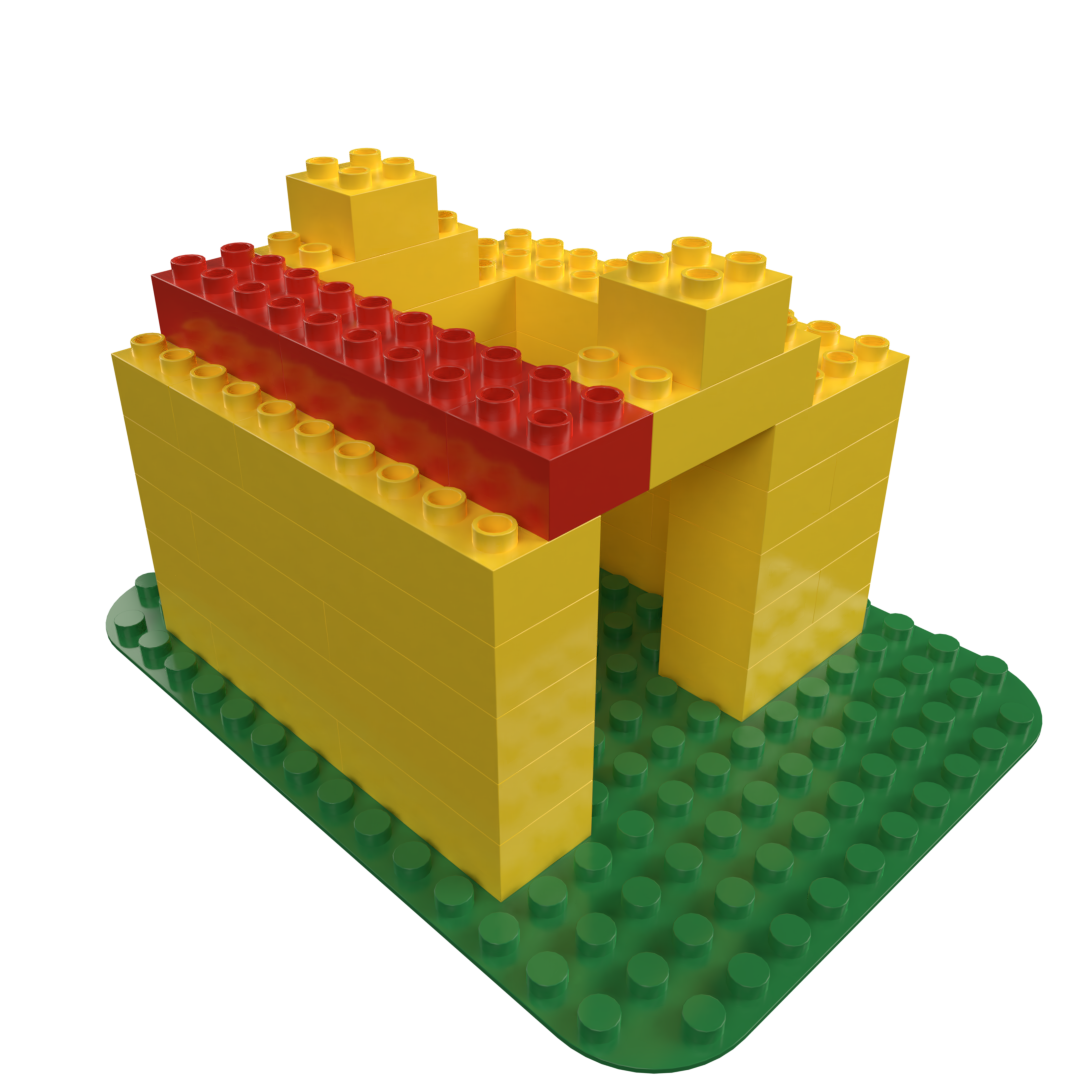
\includegraphics[width=0.7\textwidth]{images/03_transformation_framework/duplo_house_roof_step.png}
        \end{column}
    \end{columns} 
\end{frame}

\begin{frame}{What do we need?}
    \centering
    \begin{tikzpicture} 
    \path
    (-3,4) node[circle,draw,minimum size=10mm,inner sep=0pt](ME) {$E$}
    (-4.5,2) node[circle,draw,minimum size=10mm,inner sep=0pt](MA) {$M_A$}
    (-1.5,2) node[circle,draw,minimum size=10mm,inner sep=0pt](MB) {$M_B$}
    (-3,0) node[circle,draw,minimum size=10mm,inner sep=0pt](MAB) {$M_{AB}$}
    
    (3,4) node[circle,draw,minimum size=10mm,inner sep=0pt](GN) {$N$}
    (1.5,2) node[circle,draw,minimum size=10mm,inner sep=0pt](GA) {$G_A$}
    (4.5,2) node[circle,draw,minimum size=10mm,inner sep=0pt](GB) {$G_B$}
    (3,0) node[circle,draw,minimum size=10mm,inner sep=0pt](GAB) {$G_{AB}$};
    
    \path[]		
    (ME) [-, black, out=240, in=90] edge node[above] {} (MA)
    (ME) [-, black, out=300, in=90] edge node[above] {} (MB)
    
    (MA) [-{Latex[width=5]}, black, out=270, in=90] edge[onslide=<2->{red}] node[above] {} (MAB)
    (MB) [-{Latex[width=5]}, black, out=270, in=90] edge[onslide=<2->{red}] node[above] {} (MAB)
    
    (GN) [-, black, out=240, in=90] edge node[above] {} (GA)
    (GN) [-, black, out=300, in=90] edge node[above] {} (GB)
    
    (GA) [-{Latex[width=5]}, black, out=270, in=90] edge[onslide=<3->{red}] node[above] {} (GAB)
    (GB) [-{Latex[width=5]}, black, out=270, in=90] edge[onslide=<3->{red}] node[above] {} (GAB)
    
    (ME) [-{Latex[width=5]}, black, out=25, in=155] edge node[above] {$f$} (GN)
    (GN) [-{Latex[width=5]}, black, out=165, in=15] edge node[above] {} (ME)
    
    (MA) [-{Latex[width=5]}, black, out=35, in=145] edge node[above] {$f_A$} (GA)
    (GA) [-{Latex[width=5]}, black, out=155, in=25] edge node[above] {} (MA)
    
    (MB) [-{Latex[width=5]}, black, out=35, in=145] edge node[above] {$f_B$} (GB)
    (GB) [-{Latex[width=5]}, black, out=155, in=25] edge node[above] {} (MB)
    
    (MAB) [-{Latex[width=5]}, black, out=25, in=155] edge[onslide=<4->{red}] node[above] {$f_{A} \sqcup f_{B}$} (GAB)
    (GAB) [-{Latex[width=5]}, black, out=165, in=15] edge[onslide=<4->{red}] node[above] {} (MAB)
    ;
    \end{tikzpicture}
\end{frame}

\begin{frame}{What do we need?}
    Type level:
    \begin{itemize}
        \item The combination of type models
        \item The combination of type graphs
        \item The combination of transformation functions between type models and type graphs
    \end{itemize}
    \vspace{0.25cm}
    Instance level:
    \begin{itemize}
        \item The combination of instance models
        \item \alert<2>{The combination of instance graphs}
        \item The combination of transformation functions between instance models and instance graphs
    \end{itemize}
\end{frame}

\note{
	\begin{itemize}
	    \item Explain that to make the transformation framework work, some things need to be defined and proven.
	    \item Explain that the combination of models and graphs is needed.
	    \item Explain that the combination of transformation functions is needed.
	    \item Explain that both are done twice, one time for the type level and one time for the instance level.
	\end{itemize}
}

\begin{frame}{Revisiting instance graphs}
Suppose an instance graph IG typed by type graph TG:
\begin{equation*}
    IG = \langle N, E, ident \rangle
\end{equation*}\pause
\vspace{0.5cm}
Structural properties:
\begin{itemize}
    \item The set of nodes is a subset of the set of valid GROOVE nodes.
    \item The set of edges is a set of triples, with a source node, edge type and target nodes: $E \subseteq N \times ET_{TG} \times N$
    \item The $\mathrm{ident}$ function maps a set of identities to a node in the graph.
\end{itemize}
\end{frame}

\begin{frame}{Revisiting instance graphs}
Suppose an instance graph IG typed by type graph TG:
\begin{equation*}
    IG = \langle N, E, ident \rangle
\end{equation*}
\vspace{0.5cm}
Validity properties:
\begin{itemize}
    \item The nodes $N$ must be properly typed.
    \item The source of each edge $e \in E_{IG}$ must be properly typed.
    \item The target of each edge $e \in E_{IG}$ must be properly typed.
    \item Abstract types cannot have instances.
    \item The outgoing multiplicity of each edge type must be adhered to.
    \item The incoming multiplicity of each edge type must be adhered to.
    \item Nodes must be contained by at most one other node.
    \item There may be no cycle between the containment edges in $E_{IG}$.
\end{itemize}
\end{frame}

\begin{frame}{Revisiting instance graphs}
\begin{columns}[c]
    \begin{column}{0.05\textwidth}
    \end{column}\begin{column}{0.3\textwidth}
        \centering
        % To use this figure in your LaTeX document
% import the package groove/resources/groove2tikz.sty
%
\begin{tikzpicture}[scale=\tikzscale,name prefix=test-]
\node[type_node] (n0) at (2.000, -1.265) {\ml{\textbf{\hspace{0.2cm}A\hspace{0.2cm}}}};
\node[type_node] (n1) at (2.000, -2.3) {\ml{\textbf{\hspace{0.2cm}B\hspace{0.2cm}}}};

\path[basic_edge, composite](n0.south -| 1.800, -2.3) -- node[lab] {\ml{y}} (n1) ;
\path[basic_edge, composite](n1) -- node[lab] {\ml{x}} (n0.south -| 2.200, -1.265) ;
\end{tikzpicture}

    \end{column}\begin{column}{0.3\textwidth}
        \centering
        % To use this figure in your LaTeX document
% import the package groove/resources/groove2tikz.sty
%
\begin{tikzpicture}[scale=\tikzscale,name prefix=start-]
\node[basic_node] (n0) at (0.270, -0.360) {\ml{\textbf{A}}};
\node[basic_node] (n1) at (1.210, -0.760) {\ml{\textbf{B}}};
\node[basic_node] (n2) at (0.280, -1.200) {\ml{\textbf{A}}};

\path[basic_edge] (n0)  -- node[lab] {\ml{y}} (n1) ;
\path[basic_edge] (n1)  -- node[lab] {\ml{x}} (n2) ;
\end{tikzpicture}

    \end{column}\begin{column}{0.3\textwidth}
        \centering
        % To use this figure in your LaTeX document
% import the package groove/resources/groove2tikz.sty
%
\begin{tikzpicture}[scale=\tikzscale,name prefix=invalid-]
\node[basic_node] (n0) at (0.520, -0.450) {\ml{\textbf{A}}};
\node[basic_node] (n1) at (1.350, -0.460) {\ml{\textbf{B}}};

\path[basic_edge](n0.east |- 1.350, -0.530) -- node[below] {\ml{y}} (n1) ;
\path[basic_edge](n1) -- node[above] {\ml{x}} (n0.east |- 0.520, -0.370) ;
\end{tikzpicture}

    \end{column}
\end{columns}
\end{frame}

\note{
	\begin{itemize}
	    \item Revisit instance graphs by explaining the corresponding triple in more detail. Explain that there are structural and validity properties.
	    \item Show an example of the last validity property to have some visualisation of what these properties mean.
	\end{itemize}
}

\begin{frame}{Combination of instance graphs}
\begin{align*}
\mathrm{combine}(IG_A, IG_B) = \langle&
N = N_{IG_A} \cup N_{IG_B} \\&
E = E_{IG_A} \cup E_{IG_B} \\&
\mathrm{ident}(i) =
    \begin{cases}
        \mathrm{ident}_{IG_A}(i) & \mathrm{if }\ i \in \mathrm{dom}\ \mathrm{ident}_{IG_A} \\
        \mathrm{ident}_{IG_B}(i) & \mathrm{if }\ i \in \mathrm{dom}\ \mathrm{ident}_{IG_B} 
    \end{cases}\\ \rangle
\end{align*}
\end{frame}

\note{
	\begin{itemize}
	    \item Explain the definition of instance graphs in more detail. Focus especially on the nodes and edges. Try to argue that it makes sense to just combine the nodes and edges.
	\end{itemize}
}

\begin{frame}{Combination of instance graphs}
    \begin{columns}[c]
        \begin{column}{0.05\textwidth}
        \end{column}\begin{column}{0.25\textwidth}
            \centering
            % To use this figure in your LaTeX document
% import the package groove/resources/groove2tikz.sty
%
\begin{tikzpicture}[scale=1.2, every node/.style={scale=0.6}, name prefix=contact1-]
\node[basic_node] (n0) at (2.685, -3.300) {\ml{\uline{\textit{Example}} : \textbf{Contact}\\email = "networks@example.com"\\firstName = "Networkprofessor"}};

\end{tikzpicture}

        \end{column}\begin{column}{0.05\textwidth}
            \centering
            +
        \end{column}\begin{column}{0.25\textwidth}
            \centering
            % To use this figure in your LaTeX document
% import the package groove/resources/groove2tikz.sty
%
\begin{tikzpicture}[scale=\tikzscale,name prefix=contact2-]
\node[basic_node] (n0) at (1.345, -1.595) {\ml{\uline{\textit{Example}} : \textbf{Contact}\\\textit{fav}}};
\node[basic_node] (n2) at (1.295, -2.985) {\ml{\textbf{Address}\\addressLine = "November Str. 15"\\country = "NL"}};

\path[basic_edge](n0.south -| 1.295, -2.985) -- node[lab] {\ml{addresses}} (n2) ;
\end{tikzpicture}

        \end{column}\begin{column}{0.05\textwidth}
            \centering
            =
        \end{column}\begin{column}{0.3\textwidth}
            \centering
            % To use this figure in your LaTeX document
% import the package groove/resources/groove2tikz.sty
%
\begin{tikzpicture}[scale=1.2, every node/.style={scale=0.6}, name prefix=contact-]
\node[basic_node] (n0) at (1.350, -1.600) {\ml{\textbf{Contact}\\\textit{fav}\\email = "networks@example.com"\\firstName = "Networkprofessor"}};
\node[basic_node] (n2) at (1.300, -2.990) {\ml{\textbf{Address}\\addressLine = "University Str. 15"\\country = "NL"}};

\path[basic_edge](n0.south -| 1.300, -2.990) -- node[lab] {\ml{addresses}} (n2) ;
\end{tikzpicture}

        \end{column}
    \end{columns}
\end{frame}

\begin{frame}{Combination of instance graphs}
Assume that:
\begin{itemize}
    \item $IG_A$ is a valid instance graph typed by $TG_A$.
    \item $IG_B$ is a valid instance graph typed by $TG_B$.
    \item $\mathrm{combine}(TG_A, TG_B)$ is a valid type graph.
    \item All shared identities map to the same node.
\end{itemize}

Then prove using these assumptions that $\mathrm{combine}(IG_A, IG_B)$ (typed by $\mathrm{combine}(TG_A, TG_B)$) is valid.
\end{frame}

\note{
	\begin{itemize}
	    \item Explain that within the transformation framework, a proof for the combination of instance graphs is given with the assumption that $IG_A$ and $IG_B$ are valid, as well as their combination of type graphs.
	\end{itemize}
}

\begin{frame}{Combination of instance graphs}
\begin{proof}
To prove that $\mathrm{combine}(IG_A, IG_B)$ is valid, show that each of the structural properties for a valid instance graph and all the validity properties for a valid instance graph hold.
\end{proof}
\end{frame}

\note{
	\begin{itemize}
	    \item Explain what the proof looks like. It is basically proving all the properties under assumptions.
	\end{itemize}
}

\begin{frame}{Combination of instance graphs}
The source of each edge $e \in E_{IG}$ must be properly typed:\\
$\forall e \in E_{\mathrm{combine}(IG_A, IG_B)}\!: \mathrm{type}_n \big(\mathrm{src}(e)\big) \sqsubseteq_{\mathrm{combine}(TG_A, TG_B)} \mathrm{src} \big(\mathrm{type}_e(e)\big)$
\pause

\begin{proof}
Make a case distinction. $e \in E_{\mathrm{combine}(IG_A, IG_B)} \implies e \in E_{IG_A} \lor e \in E_{IG_B}$.\\
\vspace{0.2cm}
If $e \in E_{IG_A}$, then $\mathrm{type}_n \big(\mathrm{src}(e)\big) \sqsubseteq_{TG_{A}} \mathrm{src} \big(\mathrm{type}_e(e)\big)$, since $IG_A$ is valid. Types are preserved after combination.
Furthermore, because of the definition of $\mathrm{combine}(TG_A, TG_B)$, have that $\mathrm{type}_n \big(\mathrm{src}(e)\big) \sqsubseteq_{\mathrm{combine}(TG_A, TG_B)} \mathrm{src} \big(\mathrm{type}_e(e)\big)$.\\
\vspace{0.2cm}
The case for $e \in E_{IG_B}$ is similar.
\end{proof}
\end{frame}

\note{
	\begin{itemize}
	    \item Explain one property, the source of each edge must be properly typed. Introduce the first order logic equivalent of this statement.
	    \item Show the proof. Explain that if an edge is in the combination, it was in one of the two graphs. For each case, you can proof that it is also typed correctly in the combination.
	\end{itemize}
}